\begin{figure}[ht]
\begin{center}
 \begin{ccTexOnly}

   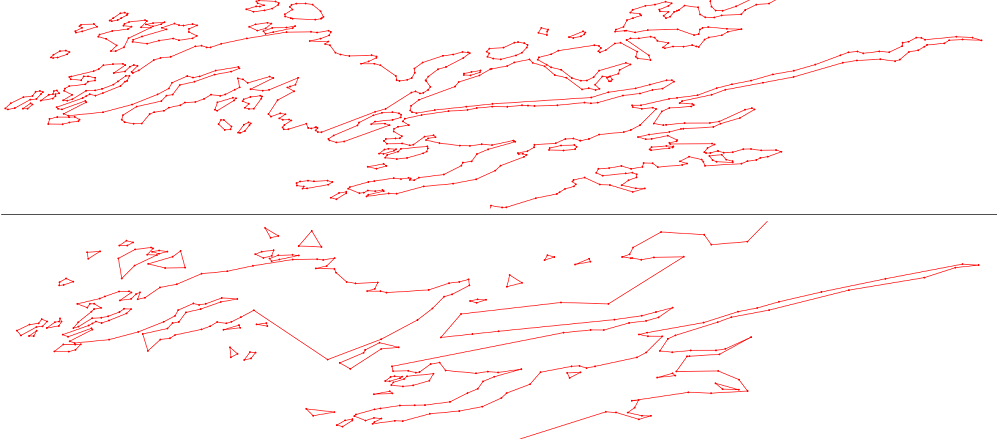
\includegraphics[height=4cm]{Polyline_simplification_2/norway.png}

 \end{ccTexOnly}
 \begin{ccHtmlOnly}
   <img border="0" src="./norway.png"><br/>
 \end{ccHtmlOnly}
 \caption{A fjord in Norway and it's simplified version.}
  \label{figure:simplified_norway}
\end{center}
\end{figure}

\section{Introduction}
Polyline simplification is the process of reducing the
number of vertices used in a set of polylines while keeping the
overall shape as much as possible.


Topology preserving polyline simplification means that neither intersections are introduced, 
nor the nesting level of a polygon changes: islands do not intersect
a simplified coastline, and islands stay in the water.

The method implemented in this package is based on
\cite{cgal:dds-scs-09}.  It can simplify any set of polylines, open or
closed, and possibly intersecting themselves or each other. The method
consists of iteratively replacing edges \ccc{(p,q)} and \ccc{(q,r)} with edge
\ccc{(p,r)} by removing the vertex $q$ from one polyline. The topology of
the polyline set is preserved during the simplification as the
algorithm guarantees that no new intersections occur as a result of
removing a vertex.

Vertices are removed according to a priority given for the vertex by a user-supplied {\em cost} function which
calculates the {\em simplification error}. The cost function is a measure of the deviation between the original polyline
and the current polyline without the vertex.

The algorithm terminates when a user-supplied {\em stop predicate} returns true, for instance,
upon reaching a desired number of vertices or reaching a maximum cost.

The polyline simplification algorithm operates on a triangulation class from 
Chapter~\ref{Chapter_2D_Triangulations}, namely \ccc{Polyline_constrained_triangulation_2<Tr>}.
This data structure allows to remove vertices of a polyline constraint, while keeping the
points of the removed vertices of the polyline constraint. The fact that it is a triangulation 
allows to perform the topology check  for vertices $p,q,r$ efficiently, as this can be decided 
based on the set of vertices adjacent to $q$ in the triangulation.


\begin{figure}[ht]
\begin{center}
 \begin{ccTexOnly}
   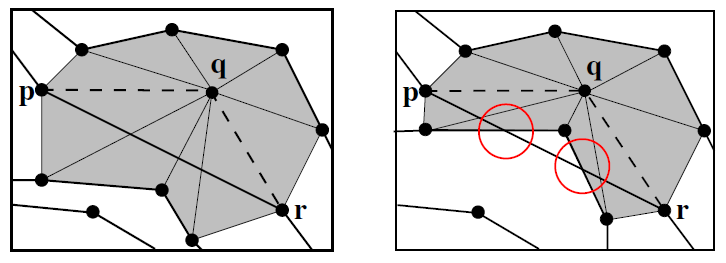
\includegraphics[height=3cm]{Polyline_simplification_2/platelet.png}
 \end{ccTexOnly}
 \begin{ccHtmlOnly}
   <img border="0" src="./platelet.png">
 \end{ccHtmlOnly}
   \label{figure:platelet}
\end{center}
\caption{Check if vertex $q$ can be removed.}
\end{figure}


\section{Cost Functions}

The specific way in which the removal cost is
calculated is called the {\em cost} function. The user can choose
different strategies by choosing a cost function object.

This package provides the three cost functions formulated in \cite{cgal:dds-scs-09}.
As the cost function is a template argument of the simplification function,
users can write and use their own.
The provided cost functions  are all based on measuring the Euclidean distance
between a subsequence of the original polyline and the corresponding subsequence of the simplified polyline
with the vertex whose cost is calculated being removed.

Let vertices \ccc{p}, \ccc{q}, and \ccc{r} be three consecutive vertices of a polyline constraint. If the vertex \ccc{q} is removed,
the edges \ccc{(p,q)} and \ccc{(q,r)} would be replaced by the
edge \ccc{(p,r)}.  


\subsection{Maximum Squared Distance}


The maximum squared distance is the maximum of the squared Euclidean distances between each 
point on the original polyline  between \ccc{p} and \ccc{r} and the line segment \ccc{(p,r)}. Let $s_0,...,s_n$ be the points strictly between \ccc{p} and \ccc{r} on the original polyline.
The cost of removing vertex \ccc{q} is: $ v_1 = \max \{ sdist((p,r), s_i) | i=0,..,n\} $

\begin{figure}[ht]
\begin{center}
 \begin{ccTexOnly}
   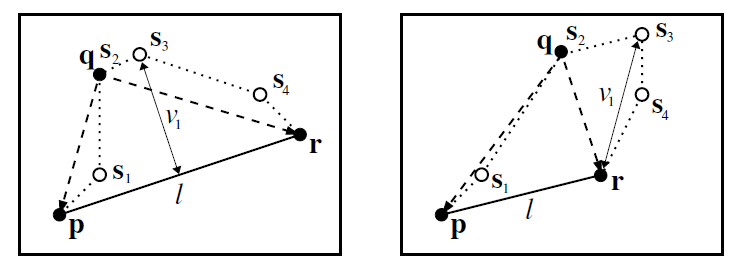
\includegraphics[height=3cm]{Polyline_simplification_2/maxDist.png}
 \end{ccTexOnly}
 \begin{ccHtmlOnly}
   <img border="0" src="./maxDist.png">
 \end{ccHtmlOnly}
   \label{figure:maxDist}
\end{center}
\caption{The maximum squared distance between \ccc{q} and \ccc{(p,r)}}
\end{figure}


\subsection{Scaled Maximum Squared Distance}

When it is important to preserve the separation of adjacent polylines, a variation of the maximum squared
distance cost can be used. Here the maximum is divided by the minimum squared Euclidean distance between
the candidate vertex \ccc{q} and all its adjacent vertices (except \ccc{p} and \ccc{r}). Those are all vertices in
adjacent polylines, or adjacent regions of the same polyline.

Let $t_0,...,t_m$ be the points of the vertices adjacent to vertex \ccc{q}, different from \ccc{p} and \ccc{r} and let $ v_2 = \max \{ sdist((p,r), t_i) | i=0,..,n\}$. The cost of removing vertex \ccc{q} is $v_1/v_2$.

This distance measure gives lower priority to vertices with close neighboring polylines.

\subsection{Hybrid Maximum Squared Distance}

The scaled maximum works well in areas with close neighboring polylines, while the absolute maximum works {\em better}
in areas where the polylines are far apart. In certain applications such as cartographic contours, there are both dense
and spare areas, so a good strategy is to use a scaled or an absolute maximum depending on the case.

The hybrid distance measure uses a parameter \ccc{R} to indicate which measure to use: if $v_2$ , i.e., the minimum distance to adjacent vertices,
is below \ccc{R}, the scaled maximum is used, otherwise the absolute maximum is used.

The cost of removing vertex \ccc{q} is  $v_1/v_2$, if $v_2 <R$, and $v_1/R$, otherwise.

As Dyken\&al.\ explain, the choice of a good value for $R$ is problem
specific.  It may depend on the pen size or the pixel size when
drawing, or on the grid size when the polyline points are on a grid.

\begin{figure}[ht]
\begin{center}
 \begin{ccTexOnly}
   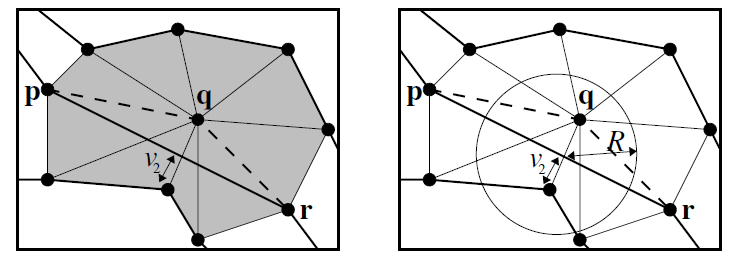
\includegraphics[height=3cm]{Polyline_simplification_2/scaledAndHybridMaxDist.png}
 \end{ccTexOnly}
 \begin{ccHtmlOnly}
   <img border="0" src="./scaledAndHybridMaxDist.png">
 \end{ccHtmlOnly}
   \label{figure:scaledAndHybrid}
\end{center}
\caption{The scaled and hybrid maximum squared distance between \ccc{q} and \ccc{(p,r)}}
\end{figure}

\newpage
\section{Examples}

The first example shows how to simplify a \ccc{CGAL::Polygon_2}.  We then show
how to simplify simultaneously several polylines, and show how to mark polyline vertices
so that they do not get removed. The last example shows how to keep, access,
and really remove points of polyline vertices that got removed by the simplification.

\subsection{Simplifying a Polygon}

The first example shows how to simplify a single polyline by halving the number of vertices.

\ccIncludeExampleCode{Polyline_simplification_2/simplify_polygon.cpp}

\newpage
\subsection{Simplifying Several Polylines}

In the second example we insert several polygons in a \ccc{Polyline_simplification_2}.  Assuming that the polygons do not intersect, we can
take the default template parameters for the \ccc{Constrained_Delaunay_triangulation_2}.

Before calling \ccc{Polyline_simplification_2::simplify} we mark some polyline vertices as not
removable.
This package provides a convenience function \ccc{Polyline_simplification_2::mark_vertices_unremovable} that marks
the vertices with smallest and largest \ccc{x} and \ccc{y} coordinates
of each polyline constraint as non-removable.
The class \ccc{Polyline_constrained_triangulation_2<Tr>}
offers functions to mark individual polyline vertices as non removable.
Finally, we iterate over all vertices of all polyline constraints.

\ccIncludeExampleCode{Polyline_simplification_2/simplify.cpp}

\newpage
\subsection{Keeping Points While Removing Vertices}

In this example we show the version of \ccc{Polyline_simplification_2::simplify}
that simplifies a single polyline constraint, and keeps
the points while removing vertices.

During the simplification the cost functions need the original
sequence of points.  
As explained in the introduction the \ccc{Polyline_constrained_triangulation_2<Tr>} allows to remove vertices from a polyline constraint,
and hence from the triangulation, while keeping the
point in the polyline constraint. This explains why there is
a \ccc{Vertex_in_constraint_iterator} and a 
\ccc{Point_in_constraint_iterator}.

With the last argument of \ccc{Polyline_simplification_2::simplify} set 
to \ccc{true}, we can keep the points even when
the simplification function has returned. 
We might want to keep them, 
because we want to call \ccc{Polyline_simplification_2::simplify} once again
for the same polyline constraint, while measuring the simplification
error against the original polyline.

The print function traverses each polyline constraint
twice. First to print the points on the simplified polyline, and
then to print the points of the original polyline.

At< the end we remove the points that were kept from the constraints.

\ccIncludeExampleCode{Polyline_simplification_2/points_and_vertices.cpp}


\section{Design and Implementation History}

Dyken et al \cite{cgal:dds-scs-09} combine a classical polyline simplification algorithm
with the triangulation of polylines in order to check if an elementary simplification step can be
performed. In our implementation we simplified this test even further. 

Fernando Cacciola made a first prototype implementation for GeometryFactory, and Andreas Fabri
developed the \ccc{Polyline_constrained_triangulation<Tr>} and the final version of this package.



